% !TEX root = ./main.tex
\chapter{Frontend Unity e Logica Applicativa}
\label{app:frontend}

Questa appendice guarda più da vicino il lato client di SOULFRAME. L'attenzione è sul frontend Unity come luogo in cui si tengono insieme stato applicativo, onboarding dell'utente e gestione concreta del turno conversazionale.

\section{Architettura client e stato applicativo}
Nel frontend, la centralità di \texttt{UIFlowController} non significa che tutto il lavoro ricada su una sola classe. La soluzione si distribuisce invece su alcuni componenti che, letti insieme, mostrano abbastanza bene la forma applicativa del client.

\par\begingroup
\scriptsize
\setlength{\LTleft}{0pt}
\setlength{\LTright}{0pt}
\captionsetup{type=table}
\captionof{table}{Componenti principali del frontend Unity.}
\label{tab:appendix-frontend-components}
\begin{longtable}{|>{\raggedright\arraybackslash}p{0.33\textwidth}|>{\raggedright\arraybackslash}p{\dimexpr0.67\textwidth-4\tabcolsep-3\arrayrulewidth\relax}|}
\hline
\textbf{Classe} & \textbf{Funzione nel client} \\
\hline
\endfirsthead
\hline
\textbf{Classe} & \textbf{Funzione nel client} \\
\hline
\endhead
\texttt{UIFlowController} & Governa la macchina a stati, le transizioni principali, le richieste backend e la logica di \texttt{MainMode}. \\
\hline
\texttt{AvatarManager} & Coordina selezione avatar, import backend-driven, caricamento runtime dei \texttt{.glb} e wiring dei componenti embodied. \\
\hline
\path{AvatarLibraryCarousel.cs} & Gestisce libreria, preview asincrone, selezione e conferma del profilo attivo. \\
\hline
\path{AvaturnULipSyncBinder.cs} & Costruisce a runtime il mapping viseme$\rightarrow$blendshape per gli avatar importati. \\
\hline
\path{AvaturnIdleLookAndBlink.cs} & Introduce blink, micro-movimenti e gestione dello sguardo in idle, listening e speaking. \\
\hline
\end{longtable}
\par\endgroup

Letta così, la tabella rischia di sembrare una semplice mappa di classi. In realtà mostra una divisione del lavoro abbastanza netta: \texttt{UIFlowController} tiene insieme il ciclo applicativo, \texttt{AvatarManager} si occupa del profilo embodied e del suo caricamento, mentre i componenti più specifici entrano in gioco solo quando quel profilo deve diventare un avatar davvero usabile in scena.

\paragraph{Macchina a stati e gating del profilo.}
Il client si muove attorno a sei stati: \texttt{Boot}, \texttt{MainMenu}, \texttt{AvatarLibrary}, \texttt{SetupVoice}, \texttt{SetupMemory}, \texttt{MainMode}. Il punto più importante non è il numero degli stati, ma la logica di gating:

Questo disegno evita che l'utente entri direttamente in conversazione con un profilo ancora incompleto. Onboarding e bootstrap restano così parte reale del sistema, non un prologo separato.

\begin{lstlisting}[style=sfcode,language={[Sharp]C},caption={Estratto adattato da \texttt{UIFlowController.cs}: scelta dello stato dopo i controlli di boot.}]
if (!coquiReady || !ragReady)
    return UIState.Boot;
if (!voiceInfo.has_voice)
    return UIState.SetupVoice;
if (statsInfo.total_memories <= 0)
    return UIState.SetupMemory;
return UIState.MainMenu;
\end{lstlisting}

\section{Gestione avatar e setup voce}
Nel client questo è il punto in cui profilo avatar e voce smettono di essere semplice configurazione e diventano prerequisiti reali dell'interazione. Per questo libreria, import, validazione del campione vocale e salvataggio del profilo restano nello stesso blocco.

\paragraph{AvatarManager e libreria avatar.}
\texttt{AvatarManager} mantiene separati tre problemi:
\begin{itemize}
\item come ottenere il riferimento a un avatar;
\item come normalizzare URL e sorgenti tra locale e deploy pubblico;
\item come istanziare il modello in scena e completarne il wiring.
\end{itemize}

Nel percorso importato, il manager riceve un payload JSON dal bridge Avaturn, invia \texttt{/avatars/import} al backend e ottiene un \texttt{cached\_glb\_url}. Solo a quel punto scarica il file dal proprio backend e lo istanzia con GLTFast. Nel percorso locale, invece, usa i modelli di fallback già previsti nel progetto.

\begin{lstlisting}[language=json,style=sfpayload,title={Import avatar backend-driven},caption={Payload minimo osservabile nel passaggio tra export Avaturn e catalogo del backend.}]
POST /avatars/import
{
  "url": "https://api.avaturn.me/avatars/exports/.../model",
  "gender": "male",
  "bodyId": "body_1",
  "urlType": "httpURL"
}

200 OK
{
  "avatar_id": "019c8296-1a77-75b1-9d4b-c36ff20d1a4c",
  "cached_glb_url": "/avatars/019c.../model.glb",
  "dedup": false
}
\end{lstlisting}

\texttt{AvatarLibraryCarousel} lavora soprattutto sulle preview. Scarica una miniatura tridimensionale dell'avatar, la inserisce in un item del carosello e rende selezionabile il profilo solo quando il modello è abbastanza pronto da non produrre un'esperienza incoerente.

Un dettaglio utile, che nel corpo starebbe stretto, è la separazione tra preview e avatar principale. \texttt{AvatarManager} usa identificatori di sessione distinti per evitare che un caricamento tardivo della preview finisca per sovrascrivere l'avatar attivo in scena. È una misura molto pratica: nel catalogo l'utente può cambiare scelta rapidamente, quindi i caricamenti asincroni devono poter arrivare ``fuori tempo'' senza corrompere lo stato corrente.

Per questo la libreria avatar non è trattata come un semplice passaggio cosmetico. Ogni scelta lì prepara già il resto della pipeline: memoria, voce, comportamento embodied e disponibilità effettiva del modello in scena. Se la preview e il caricamento principale si confondessero, l'utente non avrebbe solo un problema visivo; entrerebbe in uno stato conversazionale ambiguo.

\paragraph{SetupVoice: frase guida, filtro e salvataggio.}
Nel setup voce il client non si limita a registrare un campione. Costruisce prima una frase guida, poi filtra il materiale registrato e solo alla fine lo consegna a Coqui.

\begin{lstlisting}[basicstyle=\ttfamily\small,breaklines=true]
1. prova a generare una frase italiana con /chat
2. se la frase non e valida, usa un fallback locale
3. registra il WAV con lo stesso stack audio di MainMode
4. scarta subito campioni troppo brevi
5. invia il file a /transcribe
6. scarta trascrizioni vuote o spurie
7. calcola il match con la frase attesa
8. se il match e sufficiente:
     -> /set_avatar_voice
\end{lstlisting}

La frase guida viene chiesta al backend come una singola frase italiana naturale, con vincoli minimi su lunghezza e forma. Se il RAG non restituisce qualcosa di adatto, \texttt{UIFlowController} ricade su una frase locale già pronta. Questo evita che \texttt{SetupVoice} diventi fragile proprio nel momento in cui l'utente sta ancora completando il profilo.

Il cuore del controllo è \texttt{CalculateSimilarity}. Dopo una normalizzazione che porta il testo in minuscolo, rimuove diacritici e compatta i simboli non alfanumerici, il client combina due segnali:
\[
s = \mathrm{clip}_{[0,1]}\big(0.6 \cdot s_{\mathrm{seq}} + 0.4 \cdot s_{\mathrm{word}}\big),
\]
dove \(s_{\mathrm{seq}}\) deriva dalla distanza di Levenshtein normalizzata e \(s_{\mathrm{word}}\) dall'overlap lessicale tra i token. Anche qui i casi vuoti o troppo brevi vengono filtrati prima del confronto, quindi la normalizzazione non entra nei casi degeneri. La soglia usata nel progetto è \texttt{setupVoiceMinSimilarity = 0.7f}. Non serve a certificare l'identità del parlante: serve a scartare reference vocali troppo corte, troppo rumorose o troppo lontane dalla frase proposta.

\begin{lstlisting}[style=sfterminal,title={Esito tipico della validazione voce},caption={Il feedback che la UI costruisce prima di inviare il campione a Coqui.}]
frase attesa: "Mi chiamo Luca e oggi sto provando la mia voce."
trascrizione: "mi chiamo luca oggi provo la mia voce"
match: 82%
soglia minima: 70%
esito: upload verso /set_avatar_voice
\end{lstlisting}

\sloppy Un altro punto concreto riguarda la robustezza della coroutine. Il flag \texttt{setupVoiceCancelling} viene controllato dopo stop recording, trascrizione, match e upload, così il setup può essere interrotto senza lasciare richieste attive o side effect tardivi. Nel flusso reale questo incide parecchio sulla qualità percepita, perché evita onboarding ``appesi'' o messaggi incoerenti quando l'utente torna indietro a metà operazione.

\section{MainMode lato client e comportamento embodied}
\texttt{MainMode} tiene insieme stato UI, microfono, sessione conversazionale, playback e comportamento embodied. Letto in modo lineare, il flusso è questo:

\begin{lstlisting}[basicstyle=\ttfamily\small,breaklines=true]
ingresso in MainMode
  -> verifica prerequisiti avatar
  -> apre una sessione con /chat_session/start
  -> ascolta PTT oppure riceve input keyboard
  -> invia audio a /transcribe se il turno e vocale
  -> invia il turno a /chat con avatar_id e session_id
  -> prepara la risposta per la resa testuale e vocale
  -> avvia /tts_stream
  -> alimenta playback e lip sync dallo stesso flusso audio
\end{lstlisting}

Che il client supporti anche turni \texttt{keyboard} è importante, perché dimostra che \texttt{MainMode} non coincide con una sola gesture di input: coincide con una sessione conversazionale dell'avatar.

Dal lato client la sessione non è un metadato secondario. Serve a tenere insieme tre cose: il recap locale dei turni, il log conversazionale e la continuità tra input vocali e testuali. Per questo \texttt{BeginMainMode} apre la sessione appena il profilo è pronto, invece di aspettare il primo messaggio effettivo: il turno nasce così già dentro un contenitore coerente.

Anche la differenza tra desktop e touch va letta così. I due ambienti cambiano gesture, hint e comandi, ma non aprono due flussi diversi: PTT e tastiera sono soltanto due modi di entrare nella stessa conversazione.

Da qui entrano in gioco anche i componenti che rendono l'avatar meno ``piatto'' durante i turni. In SOULFRAME il comportamento embodied non sta a lato di \texttt{MainMode}: resta agganciato allo stesso ciclo conversazionale e ne segue gli stati. Per questo \texttt{AvaturnULipSyncBinder} non assume un naming unico dei blendshape, ma cerca a runtime candidati compatibili per i visemi principali e aggiorna i pesi in \texttt{LateUpdate}. Gli avatar non sono tutti uguali, quindi un mapping statico sarebbe troppo fragile.

Lo stesso vale per \texttt{AvaturnIdleLookAndBlink}, che non tratta sguardo e blink come animazioni decorative. Il controller cambia comportamento in base allo stato del turno -- idle, listening, speaking, focus esterno -- così il volto dell'avatar non resta neutro proprio nei momenti in cui l'utente si aspetta un segnale di presenza.

Un esempio utile del comportamento di \texttt{SetupVoice} compare quando la frase attesa non viene pronunciata in modo abbastanza aderente. In quel caso la registrazione non viene accettata e il client mostra esplicitamente che la similarità è insufficiente, invitando a riprovare.

\begin{figure}[H]
\centering
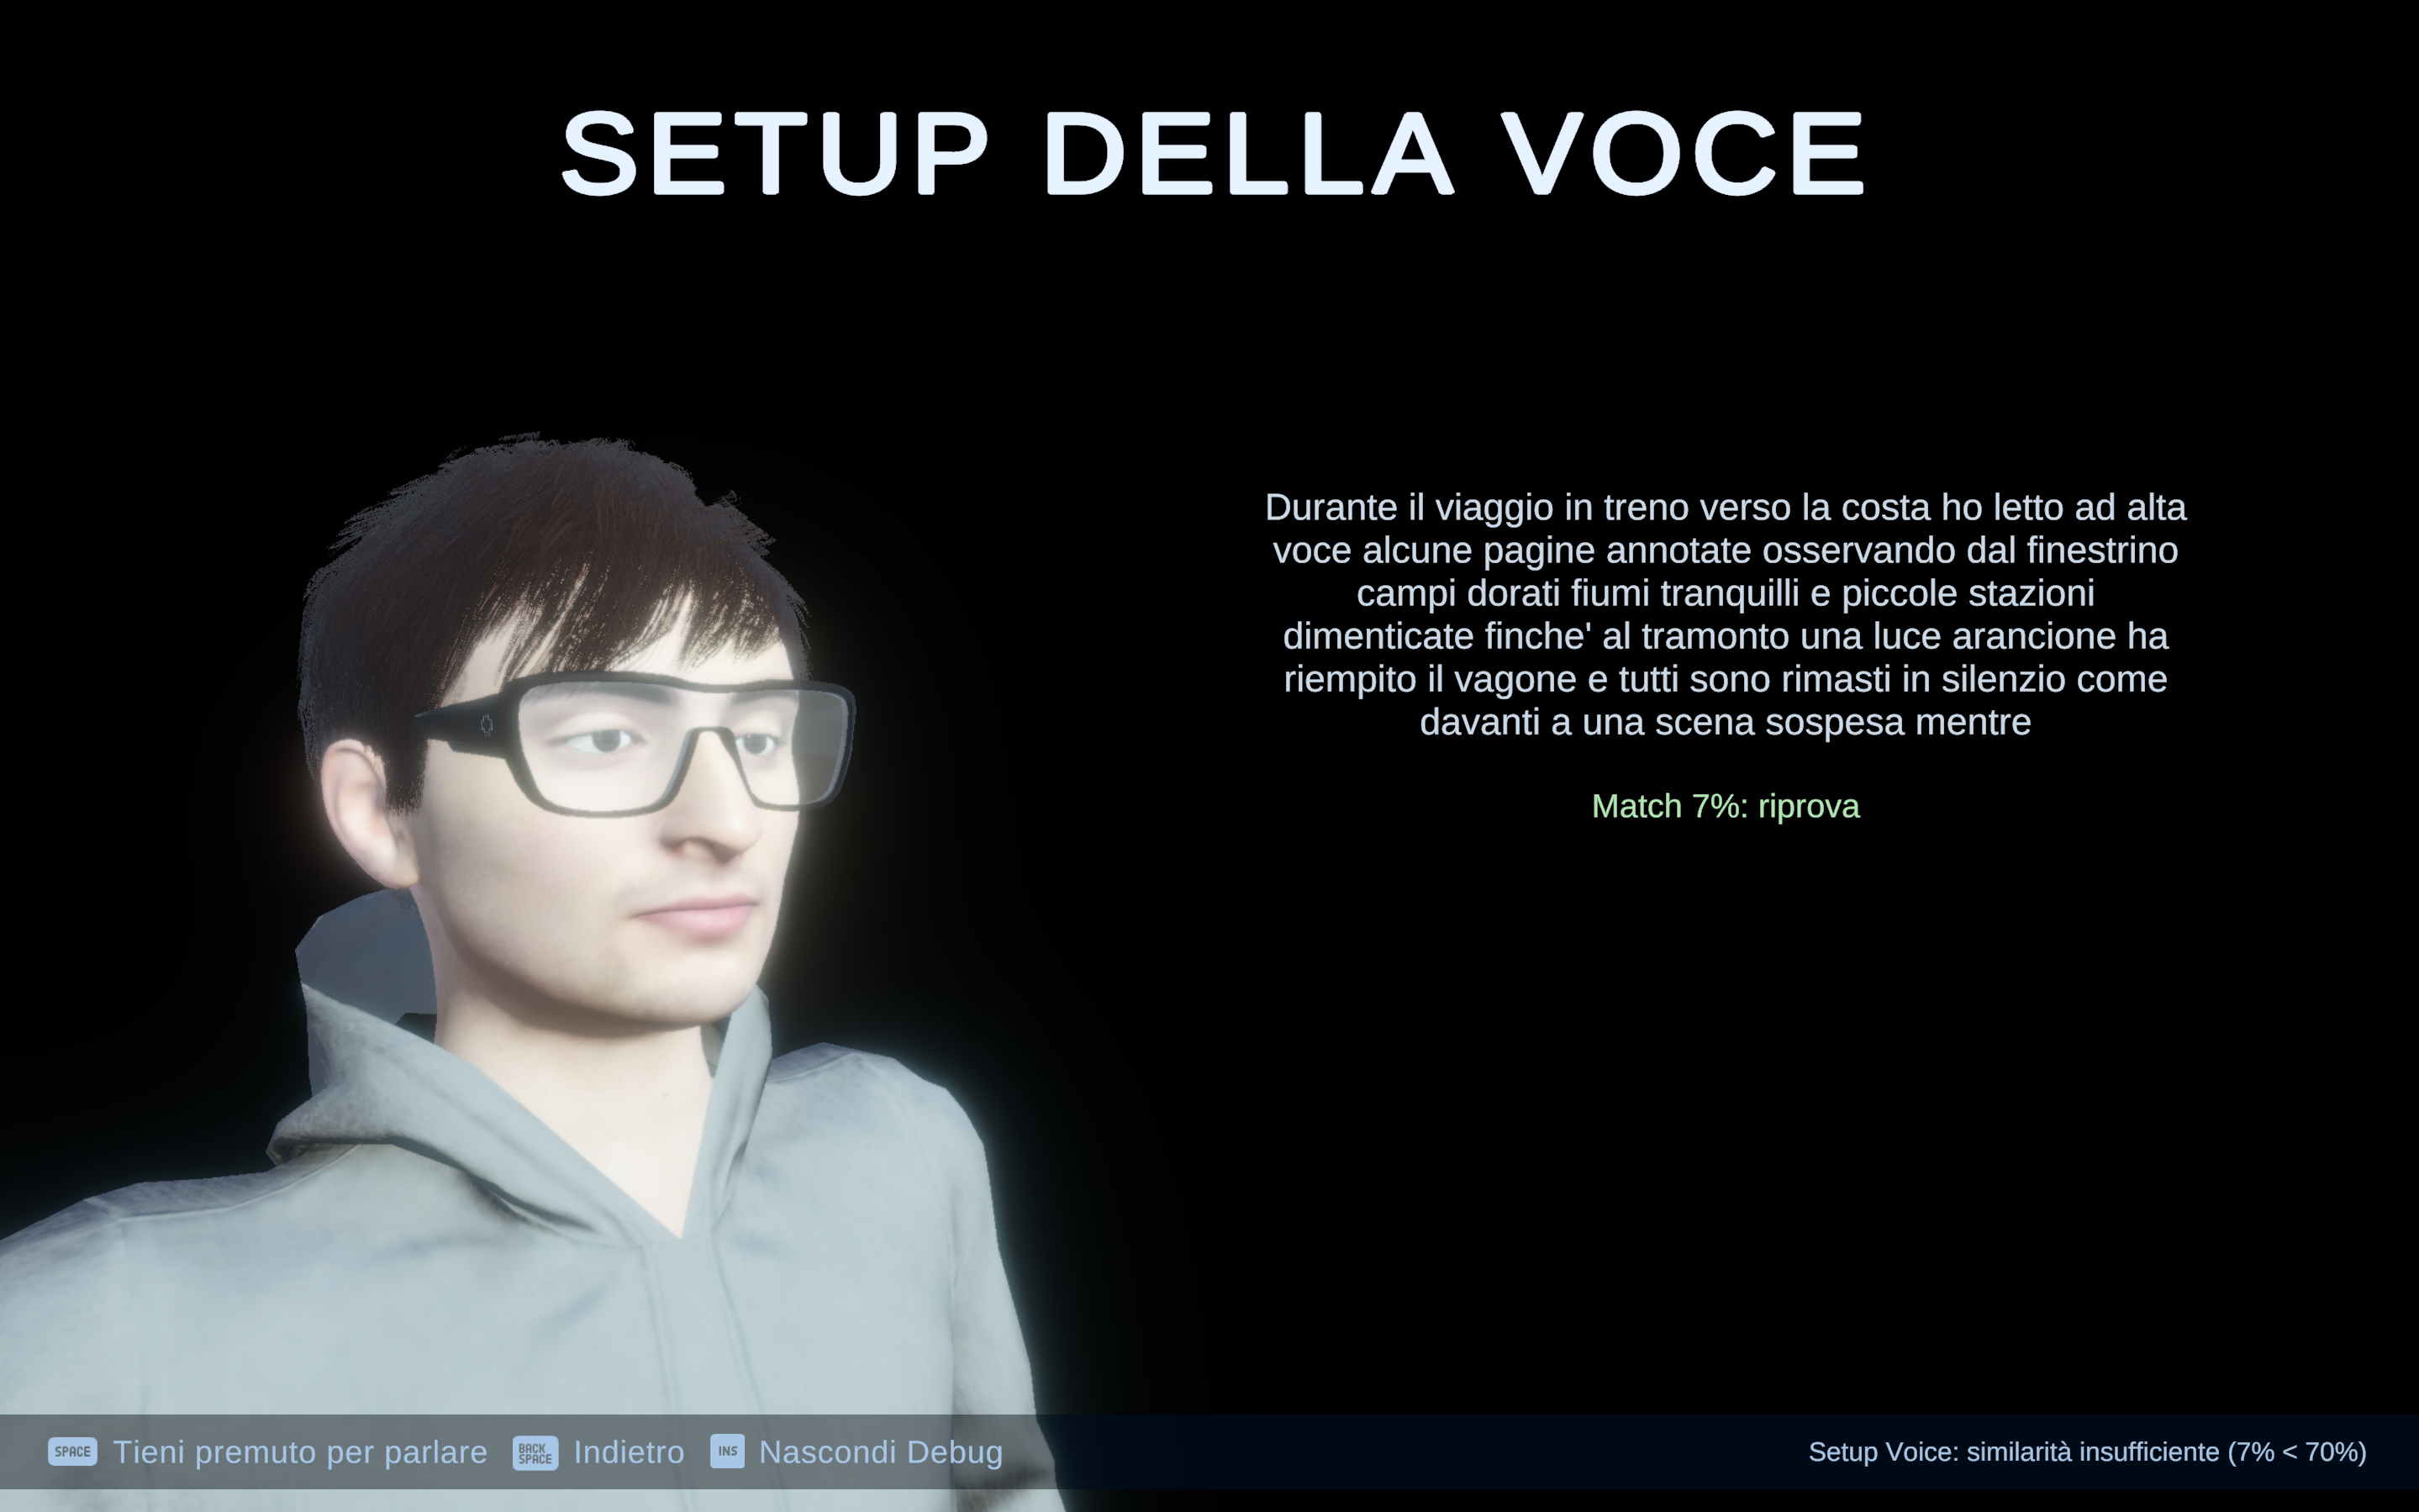
\includegraphics[width=0.92\textwidth]{Risorse/ui_setupvoice_similarity_fail.png}
\caption[Validazione fallita in SetupVoice]{Schermata di \texttt{SetupVoice} con validazione fallita: la frase pronunciata non raggiunge la soglia minima di similarità, quindi il campione vocale non viene registrato.}
\label{fig:appendix-setupvoice-fail}
\end{figure}
